\documentclass[tikz,border=2pt]{standalone}
\usepackage{amsmath}
\usepackage{amssymb}
\usepackage{xcolor}

\definecolor{journalink}{HTML}{1F1C18}
\definecolor{journalmuted}{HTML}{8A7F72}
\definecolor{journalaccent}{HTML}{9C2D2D}

\newcommand{\vennbase}{%
  \draw[journalink, line width=0.65pt, rounded corners=1pt] (-1.55,-0.95) rectangle (1.75,0.95);
  \draw[journalink, line width=0.65pt] (-0.38,0) circle (0.72);
  \draw[journalink, line width=0.65pt] (0.38,0) circle (0.72);
}

\newcommand{\shadeA}{\path[fill=journalaccent, fill opacity=0.13] (-0.38,0) circle (0.72);}
\newcommand{\shadeB}{\path[fill=journalaccent, fill opacity=0.13] (0.38,0) circle (0.72);}
\newcommand{\shadeBoth}{%
  \shadeA
  \shadeB
  \begin{scope}
    \clip (-0.38,0) circle (0.72);
    \path[fill=journalaccent, fill opacity=0.18] (0.38,0) circle (0.72);
  \end{scope}
}

\begin{document}
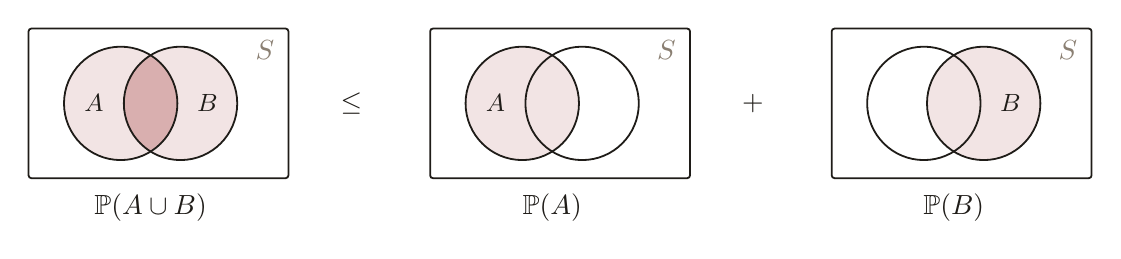
\begin{tikzpicture}[
  x=1cm,
  y=1cm,
  every node/.style={font=\normalsize}
]
  \begin{scope}[shift={(0,0)}]
    \shadeBoth
    \vennbase
    \node[journalink, font=\small] at (-0.72,0) {$A$};
    \node[journalink, font=\small] at (0.72,0) {$B$};
    \node[journalmuted] at (1.45,0.68) {$S$};
    \node[journalink] at (0,-1.32) {$\mathbb{P}(A\cup B)$};
  \end{scope}

  \node[journalink] at (2.55,0) {$\leq$};

  \begin{scope}[shift={(5.1,0)}]
    \shadeA
    \vennbase
    \node[journalink, font=\small] at (-0.72,0) {$A$};
    \node[journalmuted] at (1.45,0.68) {$S$};
    \node[journalink] at (0,-1.32) {$\mathbb{P}(A)$};
  \end{scope}

  \node[journalink] at (7.65,0) {$+$};

  \begin{scope}[shift={(10.2,0)}]
    \shadeB
    \vennbase
    \node[journalink, font=\small] at (0.72,0) {$B$};
    \node[journalmuted] at (1.45,0.68) {$S$};
    \node[journalink] at (0,-1.32) {$\mathbb{P}(B)$};
  \end{scope}
\end{tikzpicture}
\end{document}
